\documentclass[a4paper,11pt]{article}
\usepackage[left=2.5cm, right=2.5cm, top=1.5cm, bottom=1.5cm]{geometry}
\usepackage{graphicx}
\usepackage{amssymb}
\usepackage{amsmath}
\usepackage[procnames]{listings}
\usepackage{xcolor}
\usepackage[active,tightpage]{preview}
\usepackage{hyperref}

\hypersetup{ %color attributes of citation, link, etc.
    colorlinks=true,
    linkcolor=blue,
    filecolor=gray,
    urlcolor=blue,
    citecolor=blue,
}

\setlength{\parindent}{0pt}

\renewcommand{\PreviewBorder}{1in}
\newcommand{\Newpage}{\end{preview}\begin{preview}}
\newcommand{\matlab}{\textsc{Matlab}} %very important and totally necessary addition
\newcommand{\parallelsum}{\mathbin{\!/\mkern-5mu/\!}}

\newcommand\Item[1][]{%
  \ifx\relax#1\relax  \item \else \item[#1] \fi
  \abovedisplayskip=0pt\abovedisplayshortskip=0pt~\vspace*{-\baselineskip}}

%'codify' text for snippets
\usepackage{xcolor}
\definecolor{codegray}{gray}{1}
\newcommand{\code}[1]{\colorbox{codegray}{\texttt{#1}}}

\definecolor{keywords}{RGB}{255,0,90}
\definecolor{comments}{RGB}{0,0,113}
\definecolor{p_red}{RGB}{160,0,0}
\definecolor{p_green}{RGB}{0,150,0} 
\lstset{language=Python, 
        basicstyle=\ttfamily\small, 
        keywordstyle=\color{keywords},
        commentstyle=\color{comments},
        stringstyle=\color{p_red},
        showstringspaces=false,
        identifierstyle=\color{p_green},
		procnamekeys={def,class}}

\graphicspath{ {./images/} }
           
\begin{document}
\begin{preview}
\title{\LARGE{\textbf{ENGR222 Assignment 1}}}
\author{Niels Clayton : 300437590}
\date{}
\maketitle
\hrule

\begin{enumerate}
    \item Consider the parametric equation: $$ (x,y) = (8sin(t), 2t-sin(2t)) $$ over the interval $ 0 \leq t \leq 2\pi $

    \begin{enumerate}
        \item Determine the location at $ t=0 , \frac{\pi}{4}, \frac{\pi}{2}, \frac{3\pi}{4}, \pi, \frac{5\pi}{4}, \frac{3\pi}{2}, \frac{7\pi}{4}, 2\pi$ and use this to draw a rough sketch of the curve.
        
        % Insert image
        \begin{center}
            \fbox{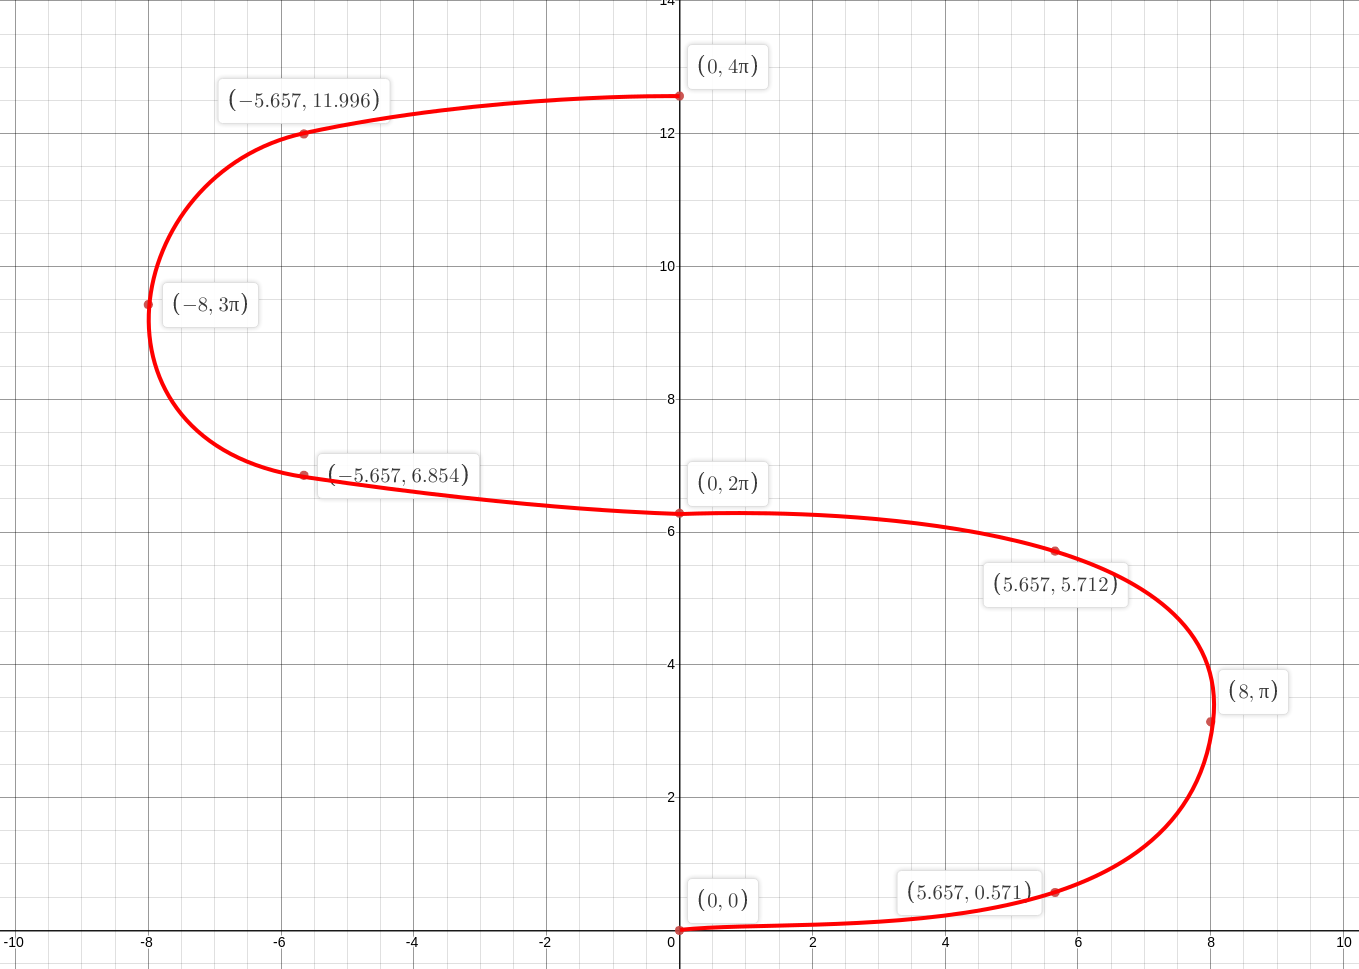
\includegraphics[width=0.8\textwidth]{image1.png}}
        \end{center}

        \item Find the unit tangent vector to the curve when $t = \frac{\pi}{6} $

        % Equation align
        \begin{align*}
            \left(f'(t), g'(t)\right) &= \left( 8 cos(t), 2 - 2 cos(2t)\right)\\
            t = \frac{\pi}{6} : \left(f'(t), g'(t)\right) &= (6.928203, 1)\\
        \end{align*}

        Calculate the unit tangent vector:
        \begin{align*}
            \frac{(f'(t), g'(t))}{||(f'(t), g'(t))||} &= \frac{(6.928203, 1)}{\sqrt{6.928203^2 + 1}} = \left( \frac{6.928203}{7}, \frac{1}{7}\right)\\
        \end{align*}

        \item Determine an equation describing the tangent line at $t = \frac{\pi}{6}$
        
        \begin{align*}
            &= \left( f(t), g(t) \right) + t \frac{(f'(t), g'(t))}{||(f'(t), g'(t))||}\\
            &= (4, 0.181) + t \cdot \left( \frac{6.928203}{7}, \frac{1}{7}\right)\\
            &= \left( \frac{6.928203 \cdot t}{7} + 4, \frac{t}{7} + 0.181 \right)
        \end{align*}

        \item Determine an equation describing the normal line at $t = \frac{\pi}{6}$

        \begin{align*}
            &=
        \end{align*}

    \end{enumerate}

    \item
\end{enumerate}


\end{preview}
\end{document}


% Equation align
\begin{align*}
    f_p &= \frac{f_c}{K_c}\\
        &= \frac{1023}{1}\\
        &= 1023\\
\end{align*}

% Insert image
\begin{center}
    \fbox{\includegraphics[width=0.9\textwidth]{image_name.png}}
\end{center}

% Insert code
\begin{center}
    \fbox{\lstinputlisting[language=Python, linerange={5-30}]{../Lab_2.m}}
\end{center}